\documentclass[10pt,oneside,openright, a4paper]{memoir}
%\usepackage{createspace} %\usepackage[size=pocket,noicc]{createspace}
%\usepackage[paperwidth=4.25in, paperheight=6.875in,bindingoffset=.75in]{geometry}
\usepackage[T1]{fontenc}
%\usepackage[latin1]{inputenc}
\usepackage{listings}
\lstset{numbers=none,boxpos=c}
\usepackage{enumitem}
\usepackage{graphicx}
\usepackage{dirtree}
\usepackage{url}
\usepackage{tikz}
\usepackage{tikz-qtree}
\usepackage{caption}
%\usepackage{scrextend}
%\usepackage{mdframed}
%\usepackage{mathpazo}
%\usepackage[protrusion=true,expansion=true]{microtype}
%\usepackage{type1cm}
%\usepackage{lettrine}
\setlrmarginsandblock{2cm}{2.5cm}{*}
\setulmarginsandblock{2cm}{2cm}{*}
\checkandfixthelayout
\linespread{1.2}


\DeclareCaptionFont{white}{\color{white}}
\DeclareCaptionFormat{listing}{%
  \parbox{\textwidth}{\colorbox{gray}{\parbox{\textwidth}{#1#2#3}}\vskip-4pt}}
\captionsetup[lstlisting]{format=listing,labelfont=white,textfont=white}
\lstset{frame=lrb,xleftmargin=\fboxsep,xrightmargin=-\fboxsep}

\renewcommand{\chapnumfont}{\chaptitlefont}    % To harmonise the font sizes
\renewcommand{\chapnamefont}{\chaptitlefont}   % idem
\renewcommand{\afterchapternum}{:\quad}        % To set the line


% See the ``Memoir customise'' template for some common customisations
% Don't forget to read the Memoir manual: memman.pdf

%\title{TITLE OF BOOK}
%\author{NAME OF AUTHOR}
%\date{} % Delete this line to display the current date
%\mdfsetup{skipabove=\topskip,skipbelow=\topskip}
%\global\mdfdefinestyle{default}{%
%  linecolor=black, middlelinewidth=1pt, %
%  leftmargin=1cm, rightmargin=1cm
%}
% Todo:   Add accounting section
%          - print money
%
%% BEGIN TITLE

\makeatletter
\def\maketitle{%
  \null
  \thispagestyle{empty}%
  \vfill
  \begin{center}\leavevmode
    \normalfont
    {\huge\raggedright \@title\par}%
    \hrulefill\par
    {\LARGE\raggedleft \@author\par}%
    \vskip 1cm
%    {\Large \@date\par}%
  \end{center}%
  \vfill
  \null
  \cleardoublepage
  }
\makeatother
\author{jacky@ru.is}
\author{Jacky Mallett}
\title{Threadneedle Programming Guide}
\date{August 2013}

%%% BEGIN DOCUMENT

\begin{document}
\let\cleardoublepage\clearpage
\maketitle
\frontmatter
\null\vfill
\begin{flushleft}
\textit{Threadneedle Programming Guide}
\copyright Jacky Mallett
All rights reserved. 2015
%ISBN--INFO
%ISBN--13: 
\bigskip
\end{flushleft}
\let\cleardoublepage\clearpage

\mainmatter
\sloppy
\chapter{Introduction}
This guide explains how to add agents to Threadneedle
or modify the existing ones, as well as how to interact
with other agents using the financial system provided by the simulation.
Instructions are also
provided on specific programming topics within Threadneedle: statistic
creation and handling, adding to the main GUI using the Java FXML interface,
specifying new Charts,
overview of Threadneedle's architecture.
\par
Users who just want to modify or create agents - which
will typically be done by subclassing existing agents - can find
instructions in Chapter \ref{ch:agents}. How to add statistics to the chart
display can be found in section \ref{ch:charts}, and general instructions on 
modifying the FXML user interface in section \ref{ch:fxml}.
\section{Design Philosophy}
There are some overall design considerations embedded in the framework
that it helps to be aware of, which have implications for programming
and simulation design.
\subsection{No Equations}
Threadneedle is intended to provide as accurate a reproduction as
possible of the financial control and information mechanisms used
in modern economies. The status of all economic equations, and in particular
any that incorporate financial information is treated
as not proven.\footnote{In the Scottish Jurisprudence system there are
three possible verdicts, guilty, not guilty and not proven. The not
proven verdict is used in cases where sufficient evidence supporting either
guilt or innocence has not been provided to the satisfaction of the jury.}
Threadneedle is intended amongst other things as a tool for testing
these equations under controlled conditions which can then be
used to ascertain their accuracy or otherwise.
\subsection{All agent actions must be performed by the agent}
No economic actions are performed by default. Agents must call the
payTaxes() and payDebts() methods each step if they wish to pay
those bills.
\par
This can be problematic when running simulations if programming errors occur, 
and the simulation
is not collecting taxes or paying debts when it is expected that this
is occurring. The alternative though is that agents have no choice about
what they do, and when they do it. Both taxation and debt payments
are sensitive to the order of evaluation of actions by the agent in 
each round, for example - for example, salaries being paid before debts are
settled may cause the agent to default on a debt payment, debts before
salaries may cause salaries not to be paid, and so this is
left to the agent's programming. Be aware of it though as a potential
source of economic bugs.
\chapter{Directory Structure}
\begin{figure}[ht]
\centering
\framebox[\textwidth]{%
\begin{minipage}{0.9\textwidth}
\dirtree{%
.1 src/.
.2 Threadneedle/.
.3 classes/.
.3 Documentation/.
.3 lib/.
.3 src/.
.4 base/.
.4 charts/.
.4 core/.
.4 agents/.
.4 resources/.
.4 statistics/.
.3 ledgers/.
.2 output/.
.2 configs/.
}
\end{minipage}
}
\caption{Threadneedle directory structure}.
\label{fig:dir-structure}
\end{figure}

Figure \ref{fig:dir-structure} shows the directories installed
under Threadneedle containing the source code, documentation
and example simulation files.  Pre-defined agent classes can be found
in the \emph{src/agent} directory, and any new agents 
should also be placed in that directory. The \emph{src/resources} directory
contains the ascii fxml files used to generate the user interface,
these can be modified and specific instructions on how to do
this is provided in the FXML section below\ref{ch:fxml}.
\chapter{Agents}
\label{ch:agents}
Every economically active entity in Threadneedle is created as a
distinct, discrete agent. Although all agents inherit from the same
base class (Agent), a distinction is
made, primarily for future development purposes, between agents that
are representing companies, such as Banks, Markets, etc., and those
that represent individuals, such as Workers, Borrowers, Investors.
\par
The inheritance tree for agents is shown in
Figure \ref{fig:inheritance}. New agents which do not specialise existing
agent types should inherit directly from either of the abstract classes, 
Company or Person. 
\par
\par
\begin{figure}[ht]
\begin{center}
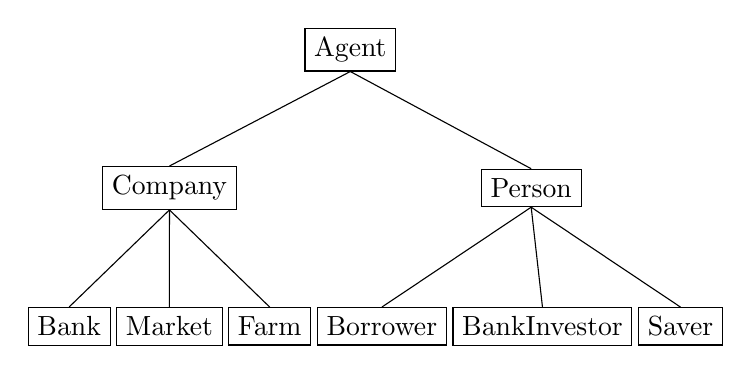
\begin{tikzpicture}[every tree node/.style=draw,level 2/.style={sibling distance = 40mm} level 3/.style={sibling distance = 5mm}]
\tikzset{level distance = 50pt}
\Tree [.{Agent}
      [.{Company} 
        {Bank}
        {Market}
        {Farm}
      ] 
      [.{Person}
        {Borrower}
        {BankInvestor}
        {Saver}
      ]
     ]
\end{tikzpicture}
\end{center}
\caption{Agent inheritance in Threadneedle}
\label{fig:inheritance}
\end{figure}
Common functionality used by both companies and people is provided
by the base Agent class.
The Company agent additionally provides mechanisms for shares to be issued,
and dividends paid on the shares, although this is not required; companies
can also exist as purely private entities. The People class on the other
hand provides support for labour employment, unemployment,  and consumption
of Needs and Wants as specified by individual simulations.
Taxation can currently be applied as a flat rate on either class of agent,
with a limit that can be set to provide a bound below which no tax is
payable.
\par
\section{Creating new agents}
\subsection{Programming}
Creating new agents is straightforward, but the steps provided below must
be followed carefully in order to integrate them correctly within the 
Threadneedle framework and to allow simulation step evaluation to work 
correctly.
\par
In order to interact correctly with the rest of the simulation,
agents must be part of the \emph{agents} packages in \emph{src/agents}
and declared \emph{public}.
\par
New agents must inherit from either the Company or Person
abstract class, and implement constructors following a pre-defined
template. Other functionality can be provided at will 
using the \emph{evaluate()} method to implement actions for the Agent
to take at each step.
\begin{enumerate}
  \item Create new java class inheriting from Company or Person
  \item Following the template in Figure \ref{lst:agent-template} add methods:
  \begin{itemize}
     \item Agent constructor for gui
     \item Agent constructor for json (saved configuration files)
     \item evaluate()
  \end{itemize}
  \item Create an icon for the agent and add it to the \emph{image} directory
  \item Add agent to the drag and drop panel by editing the threadneedle.fxml file following the template in Figure \ref{lst:fxml-agent}

\end{enumerate}
As long
as this is done correctly the
simulation framework will automagically evaluate agent behaviours each round,
keep charts updated, roll over any statistics used by the agent, and provide
access to the new agent for other agents and through the batch/command line
interface.
\par
An example of the minimum code needed to instantiate a new agent is shown 
in Figure \ref{lst:agent-template}.
\begin{lstlisting}[caption={Example Agent},label={lst:agent-template} ,
                   language=java,
                   basicstyle=\tiny]
package core;                        //All agents are part of the core package

import statistics.*;                 // Required if agent is using statistics
import static statistics.Statistic.Type
import static base.Base.*;           // Required for access to base functions

import com.google.gson.annotation.Expose; // Required to save simulation


public class ExampleAgent extends Person
{
  @Expose public long mySalary = 10;   // Exposed variables will be saved

  /**
   * Evaluation function for ExampleAgent will be called once every
   * simulation step. 
   *
   * All agent behaviours should be called from here.
   */

   protected void evaluate(boolean report, int step)
   {
      super.evaluate(report, step);    // Required to invoke framework

      // Assuming that funds are available these methods will make
      // any outstanding payments for this step.

      payDebts();                     // Make payments on all outstanding loans
      payTaxes();                     // Pay any taxes

   }

  /**
   * Constructor from GUI and CLI.
   *
   * @param name    Unique and identifying name for agent
   * @param deposit Initial bank deposit
   * @param govt    Government
   * @param bank    Bank where agent's account will be created
   */

   public ExampleAgent(String name, Govt govt, Bank bank, long deposit)
   {
      super(name, govt, bank, deposit);

      // Agent specific instantiation code can be placed here, but
      // must be duplicated in the JSON file constructor below
   }

  /**
   * No parameter constructor for loading from JSON simulation save files. 
   * All @Expose'd variables will be initialised by GSON, and it is 
   * the responsibility of the developer to set anything else correctly.
   */
  public Borrower()
  {
    super();
  }

  // Other methods may be provided or overridden as required for the agent.

}
\end{lstlisting}


\subsection{Adding Agents to the User Interface}
\label{ch:fxml}
In order to add an agent to the drag and drop user interface, once the
source code has been created and added to the \emph{src/core} directory, 
it is necessary to modify the fxml files which describe the user interface.
FXML is a powerful, but somewhat pernicty XML based UI description language 
which needs to be treated carefully.
\par
The UI fxml files are found in the \emph{src/resources} directory, with the 
general convention that the resource file name is the lower case
name of the class that instantiates it. To add a new agent, open the
\emph{src/resources/threadneedle.fxml} and add a new agent
description to the \emph{<children>} of the \emph{LeftMenu}. The recommended
approach is to copy and paste from an existing agent and modify carefuly.
Example code is shown below for the Farm agent in Figure \ref{lst:fxml-agent} 
\begin{lstlisting}[caption=Agent FXML,label=lst:fxml-agent,language=xml]
<SimNode fx:id="Farm" onDragDetected ="#mouseDragDetected"
                      onMouseReleased="#mouseDragDropped"
                      onMouseDragged ="#onDragOver">
  <image>
     <Image url="@images/F.png" preserveRatio="true" smooth="true"/>
  </image>
  <type>Farm</type>
  <tooltip>Food producer - auto-adds Food market</tooltip>
  <properties product="Food" initialDeposit="100" labourInput="5"/>
</SimNode>
\end{lstlisting}
The image file (@images/F.png) in the above example, provides the Icon displaying
the agent in the UI. The \emph{<type>} of the agent is the agent's class name, 
and \emph{<tooltip>} is the rollover help text for the agent, and
the \emph{<properties>} tag is an arbitrary set of default values which
can be provided for the Agent and be passed through to the Agent at
instantiation. 
\chapter{Statistics}
Threadneedle provides a simple statistics class which allows the
simulation and individual agents to maintain a round by round
record of selected variables. Caution is advised with the statistics
capability, since it can create scaling issues for the simulation
if too many statistics are being maintained for large numbers of agents. 
(These will typically manifest as memory issues.) Statistics can 
be visualised using the Charts package as described below.
\section{Adding Statistics}
By convention, all statistics defined in Threadneedle are prefixed 
with \emph{s\_}. There are four different types, set when the statistics
is created, which determines the operation performed by the \emph{add()}
method when used on this statistic:
\begin{description}[align=left]
\item [COUNTER] All values added to statistic are summed
\item [AVERAGE] Computes the average of values added
\item [SINGLE ]  Single value, sucessive adds() in same round overwrite value
\item [NUMBER ]  Cumulative total of add/subtracts maintained between rounds
\end{description}
\par
Statistics are managed using \emph{static} methods within the Statistic
class. To create a new Statistic assign a reference name for the statistic
and specify the type:
\begin{lstlisting}[caption=Statistic,label=lst:statistic,language=java]]
s_mkt_price = new Statistic(name, Statistic.Type.AVERAGE);
\end{lstlisting}
The constructor will check the existing statistics and 
if a statistic with that exact name already exists in the simulation,
then a reference to that statistic is returned, rather than a new
object being created. This allows statistics to be shared between
agents if required. 
\par
In order to provide a common interface between loading simulation
files and creation using the GUI, statistics initialisation is put
into its own method which is invoked by both the constructors.
\newpage
\section{Linking Charts to Statistics}
\label{ch:charts}
Charts are defined in the fxml file: \emph{src/resources/chartcontroller.fxml}.
Statistics that are used by charts should be first defined in fxml file,
and accessed using the \emph{Statistic.getStatistic(name, group, type)} 
interface, which in addition to providing support for statistics also
allows separate statistics to be part of a group shown on a single chart. 
For example:
\begin{lstlisting}[caption=Statistic fxml,label=lst:statistic-fxml,language=xml]]
<StepChart fx:id="production" title="Production" enabled = "true" 
           prefHeight="250.0" prefWidth="250.0">
   <statistics>
       <FXCollections fx:factory="observableArrayList"> </FXCollections>
   </statistics>
</StepChart>
\end{lstlisting}
The fx:id of the statistic in \emph{chartcontroller.fxml} must match the 
group specified in getStatistic(). The group specifier allows multiple
different statistics to be shown on the same chart, by using the same
group. The Statistic type and name are as explained above.
\chapter{Experiment Tagging}
Git tags are used to associate particular builds with the experiment
reports. This provides a way to cross-check experimental results
with software changes, in case the outcomes of an experiments changes
with later builds. Assuming the currently checked out branch is the
desired one to tag, then the commands to do this are:
\par
\begin{table}[ht]
\begin{tabular}{ll}
\centering
Create annotated tag: & git tag exp-b1 -m 'Builder Experiment 1' \\
List known tags:      & git tag -n \\
Checkout tag:         & git checkout exp-b1 \\
Delete tag:           & git tag -d exp-b1 \\
\end{tabular}
\end{table}
Note that in order to propagate the tag into other repositories, the
command, \emph{git push --follow-tags} must be used.
\end{document}
